Creative AI, such as using deep learning models to generate paintings and music, has been a popular research domain. Since creative activities are representative of unique human intelligence, numerous works have attempted to replicate the creative process on machines.
For example, Pharmako-AI \citep{allado-mcdowell_okojie_2020} is a book co-written by K Allado-McDowell and GPT-3 \citep{gpt3} through exchanges between the human and the language model. 
Works like DALL-E, GLIDE, and DALL-E 2 tackle the problem of synthesizing images from short language descriptions, and these generative models have produced many imaginative and inspring art pieces \citep{dallePaper,glidePaper,dalle2Paper}.
These work are often motivated by the vision to create machines that can interact with people and augment human creativity.  
Our work is driven by a similar vision: how can we build systems that can be creative like humans so that AI agents and people can pariticpate in creative activities together and inspire each other. 

\begin{figure*}[!htb]
\centering
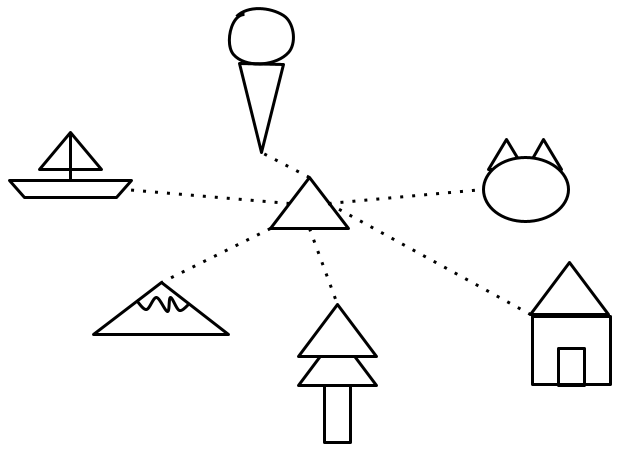
\includegraphics[width=.3\linewidth]{introduction/sketch_composition.png}  
\caption{Sketches of different objects with the triangle shape. The objects are, from top and in clockwise order: ice-cream, cat, house, pine tree, mountain, and boat.}
\label{introduction.composition}
\end{figure*}

Instead of studying how to generate realistic art works from a wide range of domains like DALL-E\todo[size=\small, color=green!20]{``a wide range of domain''?}, we approach creativity from a different angle and investigate composition of basic visual concepts to create different object sketches.
An example is illustrated in Figure \ref{introduction.composition}: a triangle can be a boat sail, a ice-cream cone, a cat ear, a house roof, a tree canopy, a mountain, etc. The same triangle is adapted to become different parts in sketches of different objects. 
While sketches do not contain all the details in natural images, they can still capture the essential features of different objects, making them simple yet widely recognizable. The abstractness allows for more creativity. 

In a similar way, language descriptors can be composed to form new concepts. For example, a \textit{large round} cat face versus a \textit{large squircle} cat face. The two faces share the same attribute \textit{large}, but one is more circular. Of course, cat face is not the only object that can be \textit{large round} or \textit{large squircle}; what object are you thinking right now that can have these attributes?
Moreover, a concept can be described in different ways. \textit{What visual features does this cat sketch have?} Some people might pick up on its usual size; others might notice its slightly edged chin, and there are still others that focus on the long whiskers curving upwards. People are likely to provide a variety of responses.  
% Word meanings shift depending on the context they are applied in. For example, the word \textit{large} in \textit{a large scoop of ice-cream} and \textit{a large cat face} implies size at different scales and conjure up different imagery. The \textit{large} scoop of ice-cream is probably oveflowing from the little cone underneath with the melting ice-cream dripping from the side, while the \textit{large} cat face implies a chubby round face compared to the cute pointy ears at the top.          

We want to build systems that can compose basic parts in a creative manner and understand how words are combined and adapted to describe different objects.  
In this thesis, we are interested in semantic parts in sketches and how people describe them. For example, a face sketch may contain four semantic parts: eyes, nose, mouth, and face contour, that can be drawn using various geometric shapes with different features.    

% % [B] 
% The ability to still get the idea across with such simple toolkit proves human creativity. We don't need complicated detailed realistic sketches, a few simple strokes are able to convey what we want to say. This type of creativity is innate. It is a creativity that we are born with: we start doodling as kids. We start scribbling on walls before knowing that we are re-creating our experience onto a canvas. It is the sort of creativity that lies on every one of us, and there is no high bar or artistic requirement to express this kind of creativity.

% % [B]
% Language creates space for imagination. Language creates room for creativity. The ambiguity in language. Large face. How large. Curved wings abstract away the details of the wings.